\documentclass{sintefbeamer}
\usepackage{amsfonts,amsmath,amssymb}
\usepackage{graphicx}
\usepackage{subcaption}
\usepackage[export]{adjustbox}
\usepackage{wrapfig}
\newcommand{\testcolor}[1]{\colorbox{#1}{\textcolor{#1}{test}} \texttt{#1}}

\usefonttheme[onlymath]{serif}

\newcommand{\hrefcol}[2]{\textcolor{cyan}{\href{#1}{#2}}}
\newcommand{\Z}{{\mathbb {Z}}}
\newcommand{\R}{{\mathbb {R}}}
\newcommand{\bb}{{\mathbf {B}}(0, 1)}
\newtheorem{remark}{Remark}

\title{Simulataneous Dilation and Translation Tilings of ${\mathbb{R}}^n$}
\subtitle{}
\author{\href{mailto:darrin.speegle@slu.edu}{Darrin Speegle} (joint with Marcin Bownik)}

\date{\today}
\titlebackground*{images/thesis_title.png}

\begin{document}

\maketitle

\begin{frame}{Tilings}

\begin{definition}
    A collection of measurable sets $\{W_j\subset \R^n: j\in J\}$ is a {\it {measurable tiling}} of ${\mathbb {R}}^n$ if 
    \begin{enumerate}
        \item $m(W_j \cap W_{{j^\prime}}) = 0$ whenever $j \not= j^\prime$, and
        \item $\bigcup_{j \in J} W_j = {\mathbb {R}}^n$ up to a set of measure zero.
    \end{enumerate}
\end{definition}
    \pause
    \begin{definition}
    Let $A$ be an invertible, $n \times n$ matrix and let $\Gamma\subset \R^n$ be a full-rank lattice.
    An {\it $(A, \Gamma)$ wavelet set} is a measurable set $W$ such that 
    \begin{itemize}
        \item $\{A^j(W): j\in \Z\}$ is a measurable tiling of $\R^n$ and
        \item $\{W + k: k \in \Gamma\}$ is a measurable tiling of $\R^n$. 
    \end{itemize}
    \end{definition}
    
\end{frame}

\begin{frame}{Examples}

1. Let $A = 2$ and $\Gamma = \Z$. The set $W = [-1, -1/2] \cup [1/2, 1]$ is an $(A, \Z)$ wavelet set.

\pause

2. Let $A = \begin{pmatrix}
    1&-1\\1&1
\end{pmatrix}$. The shaded set below is an $(A, \Z^2)$ wavelet.

\begin{figure}[h]

\begin{subfigure}{0.45\textwidth}
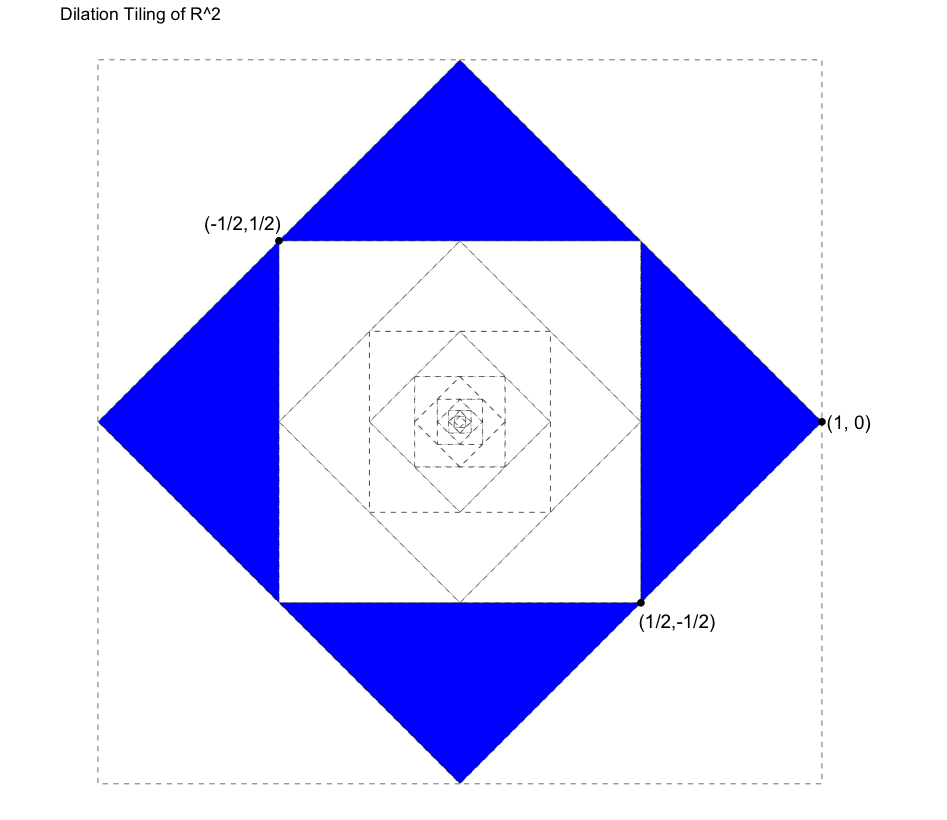
\includegraphics[width=0.9\linewidth, scale = 0.5]{images/wavelet_set_9.png} 
\end{subfigure}
\begin{subfigure}{0.45\textwidth}
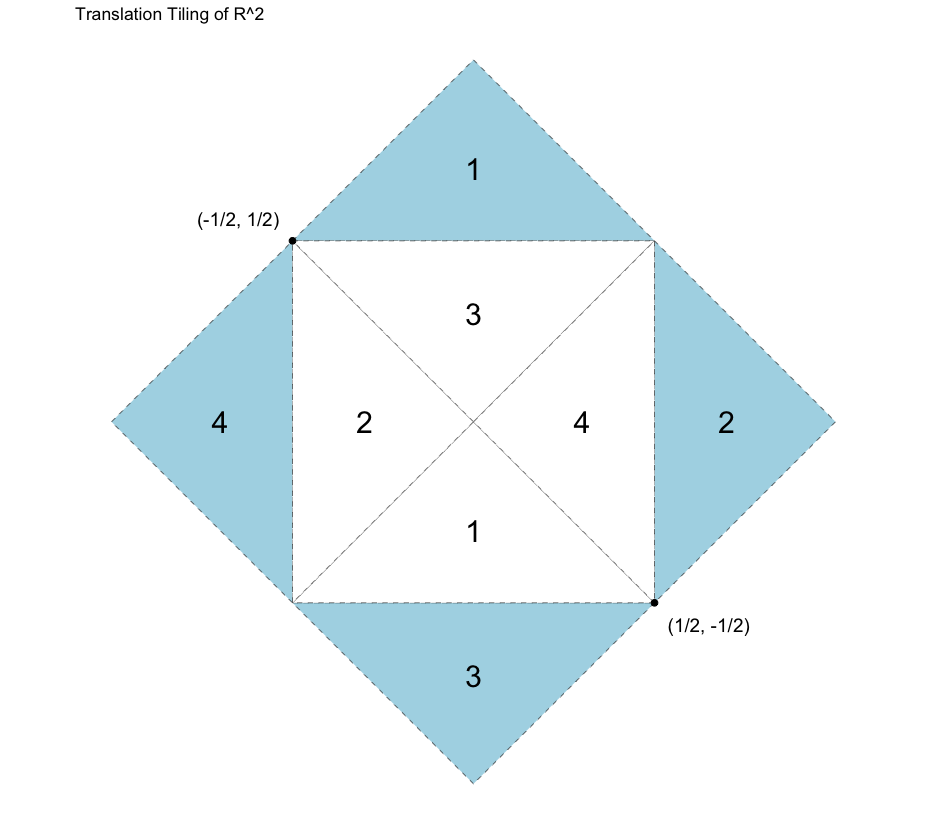
\includegraphics[width=0.9\linewidth, scale = 0.5]{images/wavelet_set_10.png}
\end{subfigure}
\end{figure}

%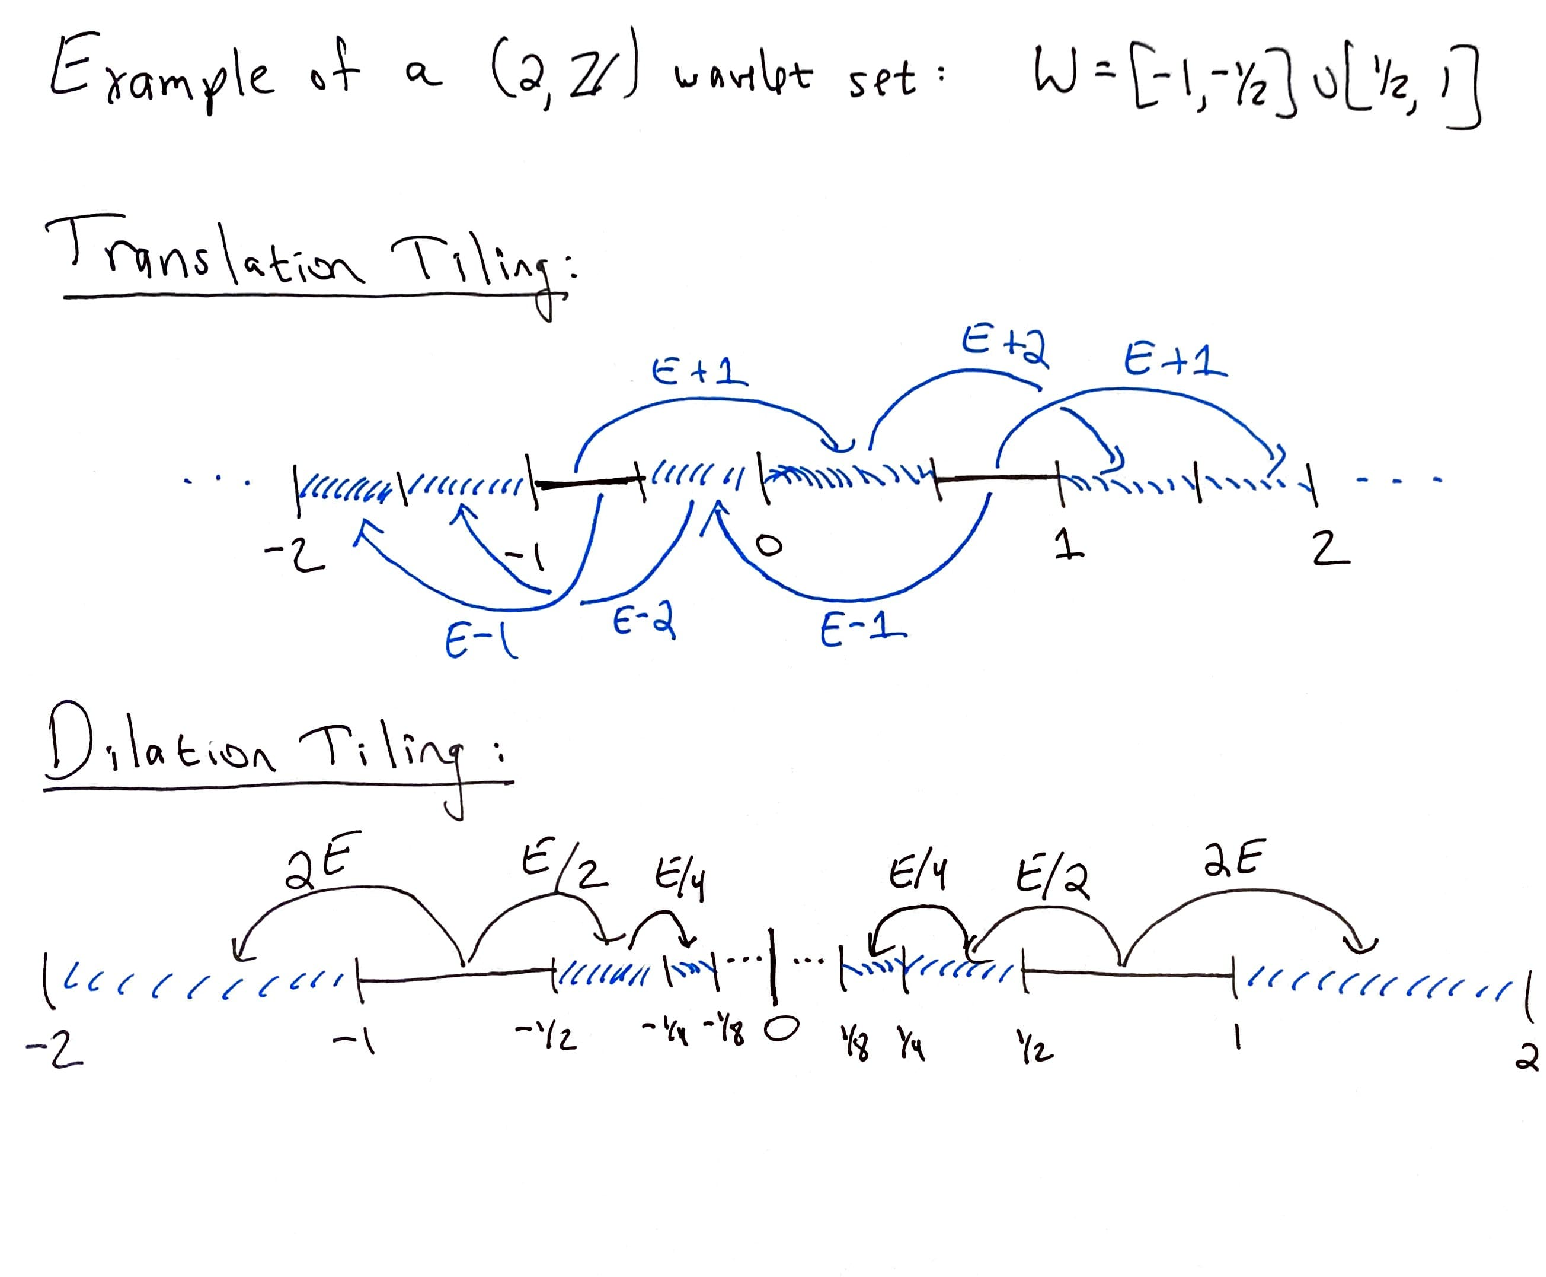
\includegraphics[width=\linewidth,height = 3.5in]{images/wavelet_1.pdf}
\end{frame}

\begin{frame}{Relationship to wavelets}

 If $W$ is an $(A, \Gamma)$ wavelet set and $\psi$ is the inverse Fourier transform of $I_W$, then $\psi$ is a $(B, \Gamma^*)$ orthogonal wavelet. That is,
    \[
    \{|\det B|^{j/2} \psi(B^j x + k): j\in \Z, k \in \Gamma^*\}
    \]
    is an orthogonal basis for $L^2(\R^n)$. Here, $B = A^T$ and $\Gamma^*$ is the dual lattice of $\Gamma$.
    
\end{frame}

\begin{frame}{Question}

{\bf{Question}} For which pairs $(A, \Gamma)$ does there exist a wavelet set?

    
\end{frame}

\begin{frame}{Source of Question}

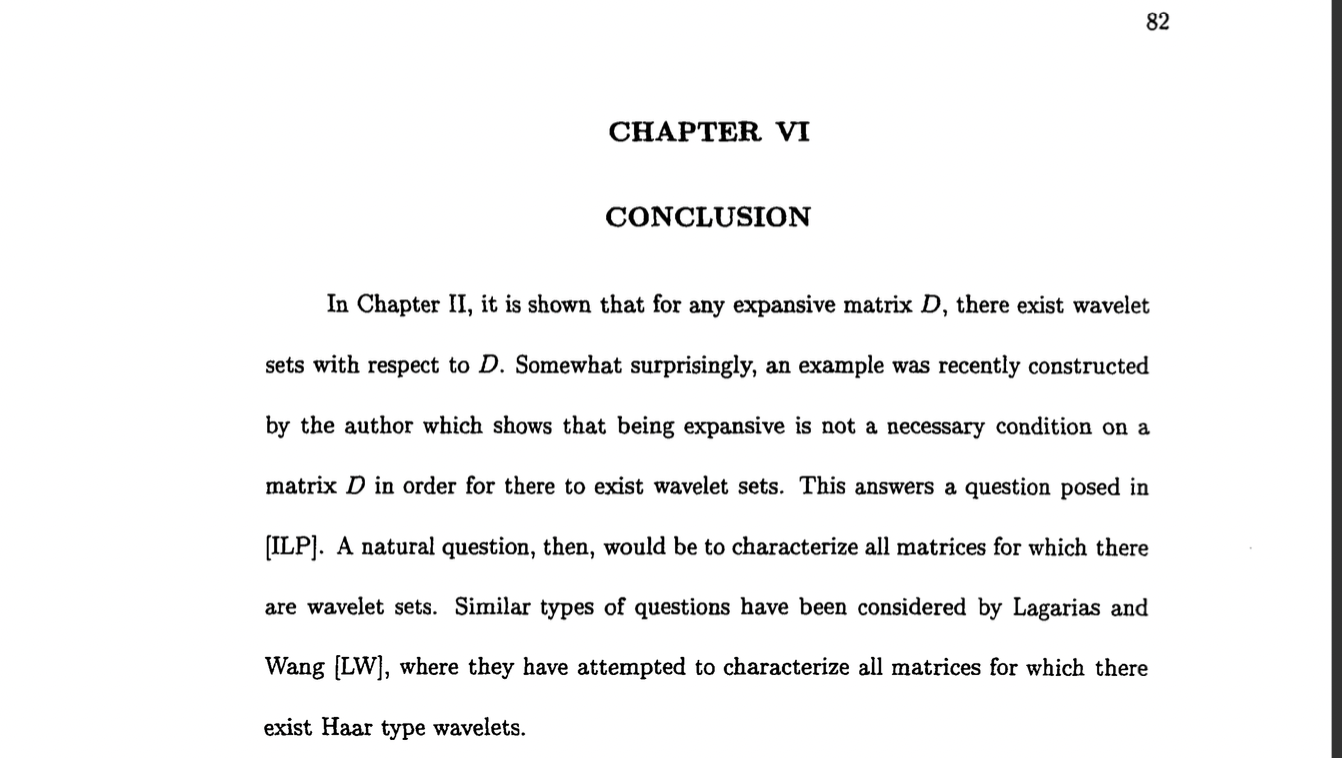
\includegraphics[width=123mm,height = 2.7in]{images/thesis_question.png}
    
\end{frame}

\begin{frame}{Me in 1995}

    
\includegraphics[width=\linewidth,height=2.7in]{images/default.jpg}

\end{frame}

\begin{frame}{Previous Results}

\begin{itemize}
    \item If $|\det A| = 1$, then no $(A, \Gamma)$ wavelet set exists. Can and will assume $|\det A| > 1$.
    
    \pause \item (Dai-Larson-S 1997) If all eigenvalues of $A$ are greater than 1 in modulus, then $(A, \Gamma)$ wavelets exist.
    
    \pause    \item (S 2004) If $A$ is $2\times 2$ and both eigenvalues are greater than or equal to one in modulus, then $(A, \Gamma)$ wavelets exist.
\end{itemize}
\end{frame}

\begin{frame}{Ionascu-Wang (2006)}
    \begin{theorem}
Let $A$ be $2\times 2$ matrix with $\left |\det A \right|>1$ and let $\Gamma$ be a full rank lattice in $\R^2$. Let $\lambda_1$ and $\lambda_2$ be the eigenvalues of $A$ such that $|\lambda_1| \ge |\lambda_2|$. There exists an $(A,\Gamma)$ wavelet set if and only if 
\begin{enumerate}[(i)]
\item $|\lambda_2| \ge 1$, or 
\item $|\lambda_2|<1$ and
$
\ker (A- \lambda_2 \mathbf I) \cap \Gamma = \{0\}.
$
\end{enumerate}
\end{theorem}

\pause 
\begin{remark}
    The key to (IW) was showing that $\ker (A - \lambda_2 \mathbf I) \cap \Gamma = \{0\}$ implies that $\liminf \#\left(A^{-j}\left(B(0, 1)\right) \cap \Gamma\right) = 1$. It turns out these are equivalent in $\R^2$
\end{remark}

        
\end{frame}

\begin{frame}{Key Object}
\begin{remark}
The key object of study is the limiting behavior as $j \to \infty$ of 
$$
\#\left(A^{-j}(B(0, R) \cap \Gamma\right)
$$
\end{remark}
\end{frame}


\begin{frame}{Higher Dimension Different}

   First noticed by Khintchine (1926), things are very different dimension 3 than dimension 2. The characterizing condition (ii) in the previous Theorem has several possible restatements in higher dimensions when the smallest eigenvalue of $A$ is less than one in modulus. For example, these four statements are all equivalent in dimension $n=2$ when $\left|\det A\right|>1$.
   
    \begin{itemize}
\item for every $R > 0$, $\liminf_{j \to \infty} \# | A^{-j}(\mathbf B(0,R)) \cap \Gamma | = 1$,
\pause \item for every $R > 0$, $\liminf_{j \to \infty} \# |A^{-j}(\mathbf B(0,R)) \cap \Gamma |< \infty$,
\pause \item for every sublattice $\Lambda\subset \Gamma$, if $V = {\operatorname{span}}(\Lambda)$ and $d=\dim V$, then
\[
\liminf_{j\to \infty} m_d(A^{-j}(\mathbf B(0,1)) \cap V) <\infty,
\]
where $m_d$ denotes the Lebesgue measure on the subspace $V$,
\pause \item if $V$ is the space spanned by the eigenvectors associated with eigenvalues less than one in modulus, then $V \cap \Gamma = \{0\}$.
        \end{itemize}  
\end{frame}

\begin{frame}{Main Result}

\begin{theorem}[Bownik-S, Am J Math, to appear]
    Let $A$ be an $n\times n$ matrix with $\left |\det A \right|>1$. Let $\Gamma \subset \R^n$ be a full rank lattice.
Then, there exists an $(A,\Gamma)$ wavelet set if and only if 
\begin{equation*}
\sum_{j=1}^\infty \frac{1}{\# \left|A^{-j}(\mathbf B(0,1)) \cap \Gamma \right |} =\infty,
\end{equation*}
\end{theorem}

\pause
\begin{remark}
    The condition above is in between 
    \begin{itemize}
\item for every $R > 0$, $\liminf_{j \to \infty} \# |A^{-j}(\mathbf B(0,R)) \cap \Gamma |< \infty$,
\item for every sublattice $\Lambda\subset \Gamma$, if $V = {\operatorname{span}}(\Lambda)$ and $d=\dim V$, then
\[
\liminf_{j\to \infty} m_d(A^{-j}(\mathbf B(0,1)) \cap V) <\infty,
\]
    \end{itemize}
\end{remark}
\end{frame}

\begin{frame}{Application}
    \begin{theorem}[Bownik-S]
Let $A$ be an $n\times n$ matrix such that $\left | \det A \right |>1$ and all eigenvalues of $A$ are greater than or equal to one in modulus. Then, for every full rank lattice $\Gamma$, there exists an $(A, \Gamma)$ wavelet set.
    \end{theorem}



\pause \begin{remark}
This is the largest class of matrices $A$ with $\left | \det A \right |>1$ for which $(A, \Gamma)$ wavelet set exists regardless of the choice of the lattice $\Gamma$.
\end{remark}
\end{frame}


\begin{frame}{Key Ingredients}
    \begin{theorem}[Margulis 1971]
Let $\Gamma$ be a full rank lattice in $\R^n$ and let $U$ be a unipotent matrix (all eigenvalues 1). There exists $\delta > 0$ such that 
$$
\liminf_{j \to \infty}  \#(U^{-j} B(0, \delta) \cap \Gamma)= 1.
$$
\end{theorem}

\pause
\begin{theorem}[Cheshmavar-F\"uhr (2020)]
     Suppose that $A$ is an $n\times n$ invertible matrix. Then, there exists a positive constant $c$ and an $n\times n$ matrix $\tilde A$ such that all eigenvalues of $\tilde A$ are positive
 and
\begin{equation*}\label{ite1}
A^j(\mathbf B(0,r/c)) \subset \tilde A^j(\mathbf B(0,r)) 
\subset A^j(\mathbf B(0,cr))
\qquad\text{for all }j\in \Z, \ r>0.
\end{equation*}
\end{theorem}

\pause
\begin{remark}
    Cheshmavar-F\"uhr allows us (essentially) to restrict to matrices with {\bf{positive}} eigenvalues.
\end{remark}

\end{frame}

\begin{frame}{Proof}
\begin{enumerate}
    \item Assume $A$ has positive eigenvalues and is in Jordan form.
\pause
      \item Write $A = \begin{bmatrix}
  A_1&0\\
  0&A_2
  \end{bmatrix}$
  where all eigenvalues of $A_1$ are larger than 1, and all eigenvalues of $A_2$ are equal to 1. Let $T$ denote the $n \times n$ matrix $T = \begin{bmatrix}
  I&0\\
  0&A_2
  \end{bmatrix}.$

%  \pause \item If $A_2$ is the identity, then $A^{-j}(B(0, 1))$ is bounded independent of $j$, and $\sum_{j=1}^\infty \frac {1}{\# \left|A^{-j}(\mathbf B(0,1)) \cap \Gamma \right |} =\infty$.
\pause \item Theorem [M] implies there exists an $\epsilon > 0$ and $n_1 < n_2 < \cdots$ such that $T^{-n_k}(B(0, \epsilon)) \cap \Gamma = \{0\}$.
  \pause \item For large $k$, $A^{-n_k}(B(0, \epsilon)) \subset T^{-n_k}(B(0, \epsilon))$, so 
  $$
  \#(A^{-n_k}(B(0, \epsilon)) \cap \Gamma) = 1 
  $$
  infinitely often, and $\sum_{j=1}^\infty \frac{1}{\# \left|A^{-j}(\mathbf B(0,\epsilon)) \cap \Gamma \right |} =\infty.$ Thus, $(A, \Gamma)$ wavelet sets exist.
\end{enumerate}
  
  
\end{frame}

\begin{frame}{Summary}

\begin{itemize}
\item Understanding the limiting behavior of $\#\left(A^{-j}B(0, 1) \cap \Gamma\right)$ is crucial to understanding when $(A, \Gamma)$ wavelet sets exist.
\pause \item There are theorems and ideas developed over the last 100 years which are useful to understand this.
\pause \item Wavelet sets exist if and only if $\sum_{j=1}^\infty \frac{1}{\# \left|A^{-j}(\mathbf B(0,1)) \cap \Gamma \right |} =\infty$
\pause \item Conjecture: $(A^T, \Gamma^*)$ orthogonal wavelets exist if and only if $\sum_{j=1}^\infty \frac{1}{\# \left|A^{-j}(\mathbf B(0,1)) \cap \Gamma \right |} =\infty$
\end{itemize}

\end{frame}

\end{document}



\begin{chapter}[]{sintefred}{Question}

For which matrix-lattice pairs $(A, \Gamma)$ does there exist a measurable set $W \subset {\mathbb{R}}^n$ such that $W$ is an $(A,\Gamma)$ wavelet set? 
\bigskip

I started working on this problem in 1995. Marcin and I announced a solution on 21 Sept, 2021.

\end{chapter}

\begin{frame}{From my thesis, 1997}

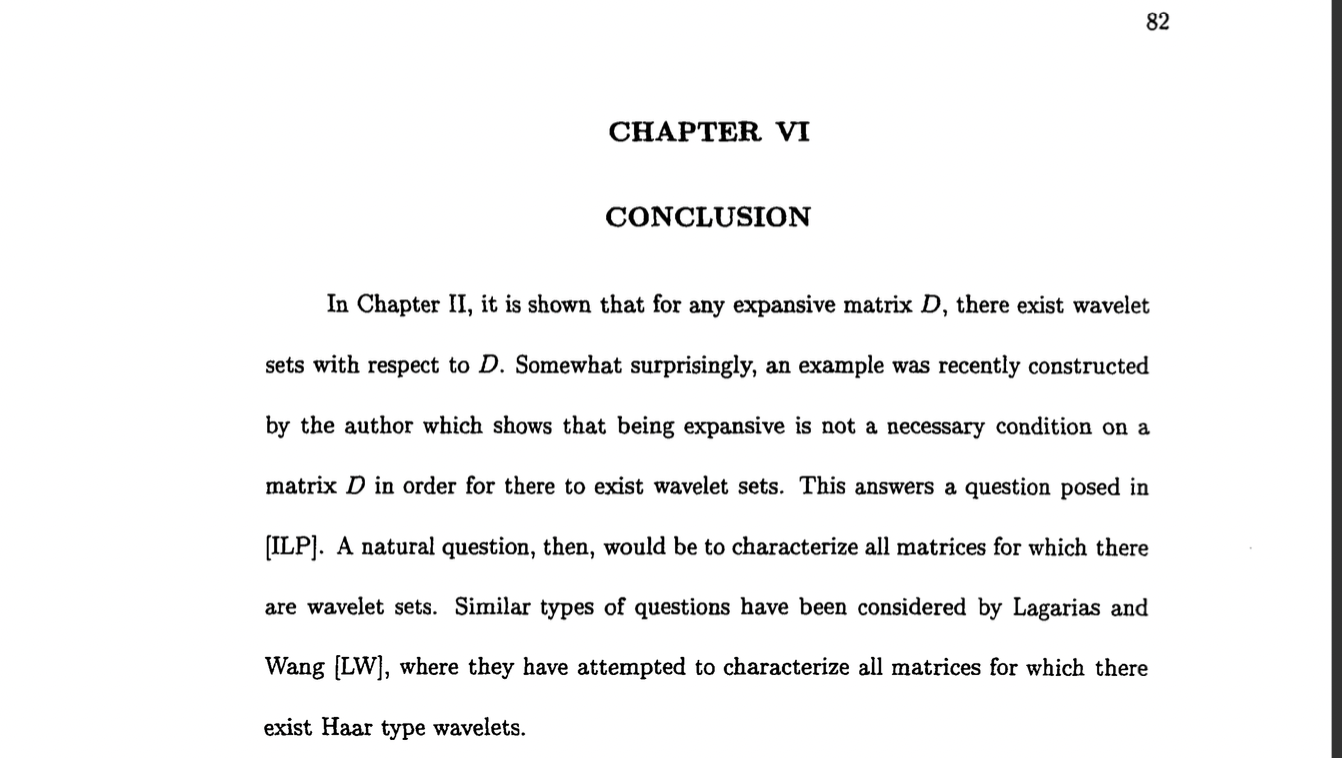
\includegraphics[width=123mm,scale=0.5]{images/thesis_question.png}

\end{frame}

\begin{frame}{Me in 1995}


\end{frame}

\begin{frame}{CodEx Organizers in 1995}

\begin{figure}[h]

\begin{subfigure}{0.3\textwidth}

\includegraphics[width=0.9\linewidth, scale = 0.2]{images/JJ.jpeg} 
\end{subfigure}
\begin{subfigure}{0.3\textwidth}
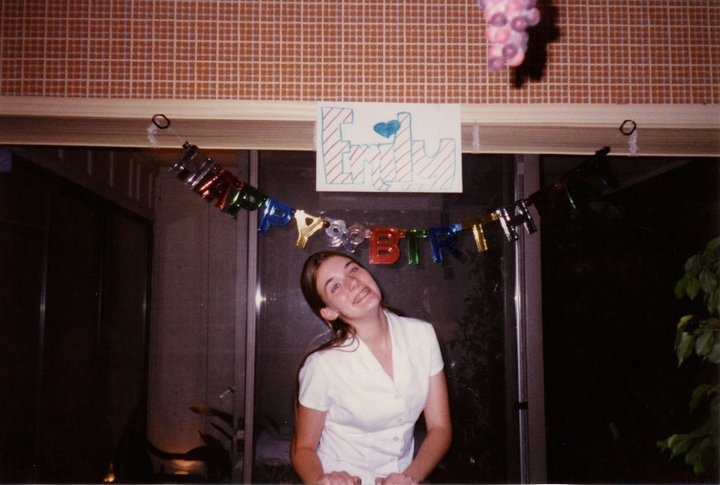
\includegraphics[width=0.9\linewidth, scale = 0.2]{images/EmPicforDarrin.jpeg}

\includegraphics[width=0.9\linewidth, scale=0.2]{images/1995_Joey_Iverson.jpg}
\end{subfigure}
\begin{subfigure}{0.3\textwidth}
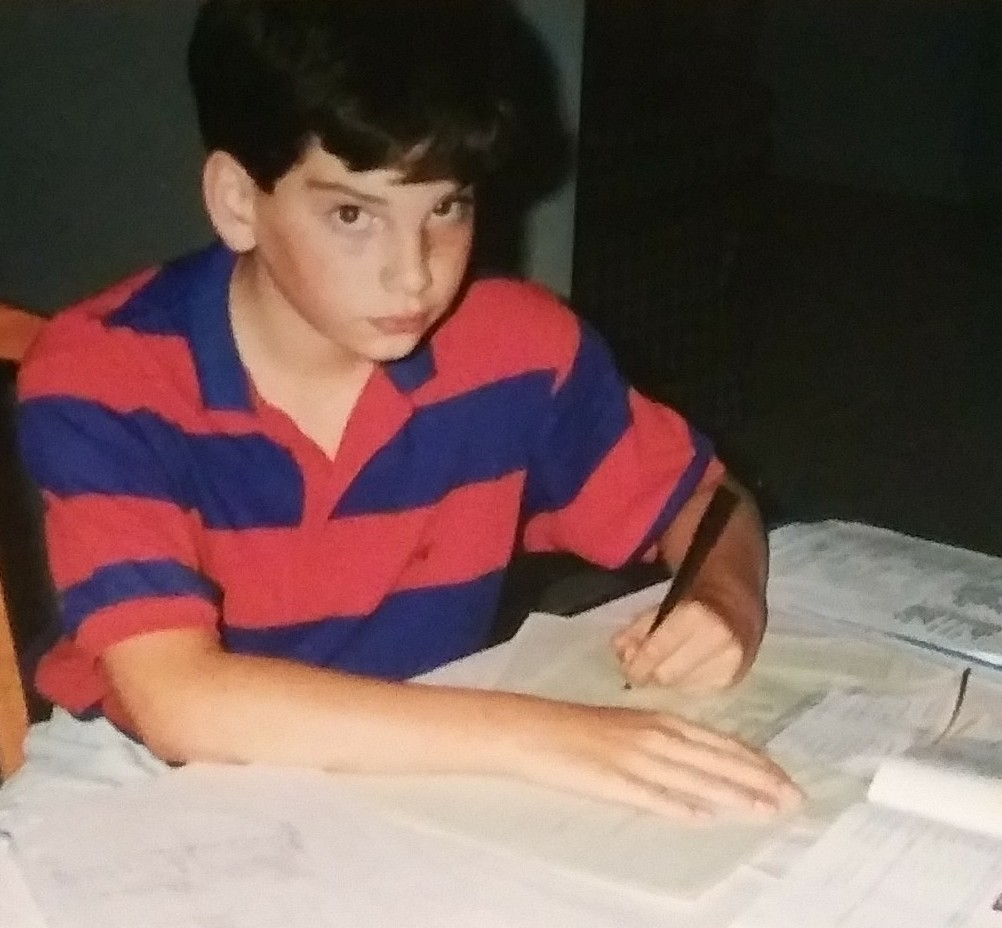
\includegraphics[width=0.9\linewidth, scale = 0.2]{images/dustin.jpg}
\end{subfigure}
\end{figure}
    
\end{frame}





\begin{frame}{First Observations}
    By a change of basis, we may {\bf{either}} assume that $\Gamma = \Z^n$ {\bf{or}} that $A$ is in real Jordan form, but not both.  You won't be missing out on much if you think of $A$ having real eigenvalues. Even the diagonal case is quite challenging. We are then forced to allow $\Gamma$ to be an arbitrary full-rank lattice.
    
    
    \pause\bigskip
    Since every $(A, \Gamma)$ wavelet set is also an $(A^{-1}, \Gamma)$ wavelet set, we can assume WLOG that $|\det A| \ge 1$.
    
\end{frame}

\begin{frame}{What about translation and dilation separately?}
    
    \begin{theorem}
      Let $\Gamma \subset \R^n$ be a full-rank lattice. There exists a measurable set $U$ such that $\{U + k: k \in \Gamma\}$ is a measurable tiling of $\R^n$. Moreover, given $\Gamma$, every such set $U$ has the same, finite measure.
      
      In particular, every $(A, \Gamma)$ wavelet set has the same, finite measure.
    \end{theorem}
    \pause
    \begin{theorem}
      Let $A$ be an invertible matrix. There exists a set of finite measure $V$ such that $\{A^j(V): j \in \Z\}$ is a measurable tiling if and only if $|\det A| \not= 1$.
      
      In particular, if $|\det A| = 1$, then no $(A, \Gamma)$ wavelet set can exist.
    \end{theorem}
\pause
\begin{remark}
 From here on, we will assume WLOG $|\det A| > 1$.
\end{remark}
\end{frame}

\begin{frame}{Main Result}
   \begin{theorem}[Bownik-S 2021]
     Let $A$ be an invertible $n \times n$ matrix with $|\det A| > 1$ and $\Gamma$ a full-rank lattice. There exists an $(A, \Gamma)$ wavelet set if and only if 
     \[
       \sum_{j = 1}^\infty \frac {1}{\#\left | A^{-j}(\bb) \cap \Gamma \right |} = \infty
     \]
     Here, $\#|\Omega|$ denotes the cardinality of the set $\Omega$.
   \end{theorem}
\end{frame}

\begin{frame}{Motivation of Condition in Main Theorem}
    
    Let $A = \begin{pmatrix} 2&0\\0&2/3 \end{pmatrix}$ and $\Gamma = \Z^2$. No $(A, \Z^2)$ wavelet set exists. Let's see why.
    
    \medskip
    
    Let $U = [1,2] \times \R$. If $W$ is an $(A, \Gamma)$ wavelet set, then $W_j := A^{-j}(U)\cap W$ satisfies the following two properties:
    
    \begin{enumerate}
        \item $m\left ((W_j + \gamma_1) \cap (W_j + \gamma_2)\right) = 0$ whenever $\gamma_1 \not= \gamma_1$. (We say the set $W_j$ packs by $\Gamma$ translations.
        \pause
        \item $\sum_{j \in \Z} m\left(A^j(W_j)\right) = \infty$.
    \end{enumerate}
    \pause
    Why 2? Because $U = \bigcup_{j \in \Z} A^j(W_j)$.
    
    \medskip
    
    \pause
    
    We show that no collection of sets $\{W_j: j\in \Z\}$ can exist that satisfy 1, 2 and $W_j \subset A^{-j}(U)$ on the next slide.
    
\end{frame}


\begin{frame}{More Motivation}
    
    By condition 1, $m(W_{-j}) \le 1$ for $j \ge 0$. Therefore, 
    \[
    \sum_{j = 0}^\infty m(A^{-j}(W_{-j})) \le \sum_{j = 0}^\infty (\det A)^{-j} = \sum_{j = 0}^\infty (4/3)^{-j} < \infty
    \]
    
    \pause
    
    
    
    
    For $ j \ge 1$, $W_j \subset A^{-j}(U)$. This and 1 imply that $m(W_j) \le 2^{-j}$. 
    
    \pause
    
    \begin{center}
    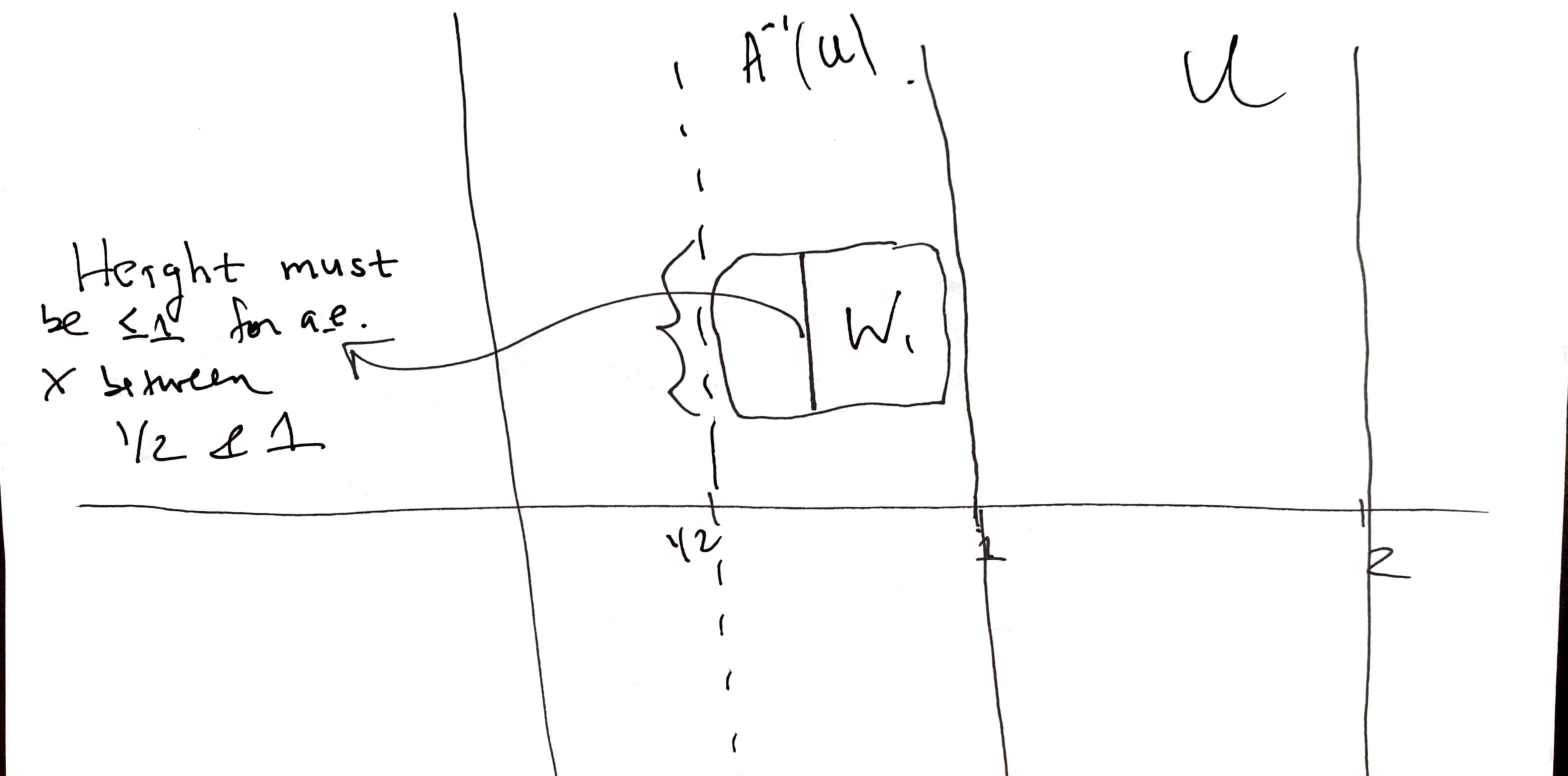
\includegraphics[width=4in,height = 1in]{images/small_obstruction.pdf}
    \end{center}    

    \pause    
    Therefore, 
    
    \[
    \sum_{j = 0}^\infty m(A^{j}(W_{j})) \le \sum_{j = 0}^\infty (\det A)^{j} 2^{-j} = \sum_{j = 0}^\infty (2/3)^{j} < \infty
    \]
    
    
\end{frame}

\begin{frame}{More Motivation}
    
    Keep $A = \begin{pmatrix} 2&0\\0&2/3 \end{pmatrix}$ and consider a general lattice $\Gamma$. How can we construct sets $W_j \subset A^{-j}(U)$ such that each $W_j$ packs by translations and $\sum_{j \in \Z} m(A^j(W_j)) = \infty$?
    
    \pause \vfill
    
    Note that for $j < 0$, we are stuck. We still have $m(W_j) \le C$, so 
    \[
\sum_{j = 0}^\infty m(A^{-j}(W_{-j})) \le \sum_{j = 0}^\infty |\det A|^{-j} C< \infty
    \]
    (Recall we assume $|\det A| > 1$.) We must look at $W_j \subset A^{-j}(U)$ for $j > 0$. 
    
    \pause \vfill
    
    Idea: Let $B$ be a Euclidean ball contained in $U$, so $A^{-j}(B) \subset A^{-j}(U)$. If $W_j \subset A^{-j}(B)$, what must be true about $m(W_j)$ to get $\sum_{j\in\Z} m(A^j(W_j)) = \infty$?
    
\end{frame}

\begin{frame}{Last One}
    
   Let $r_j = m(W_j)/m(A^{-j}(B))$. We have
\begin{align*}
    \sum_{j = 1}^\infty m(A^j(W_j)) &= \sum_{j = 1}^\infty |\det A|^j m(W_j)\\
    &= \sum_{j = 1}^\infty |\det A|^j |\det A|^{-j} m(B) r_j = m(B) \sum_{j = 1}^\infty r_j
\end{align*}
    
    \vfill
    
    {\bf{Note:}} 
    
    \[
      r_j \ge  \frac{1}{\sup \sum_{\gamma\in\Gamma} I_{A^{-j}(B)}(\cdot + \gamma)} \approx \frac{1}{\# |A^{-j}(\bb) \cap \Gamma|}
    \]
    so in order for the sum above to be $\infty$, we it suffices that
    \[
    \sum_{j = 1}^\infty \frac{1}{\# |A^{-j}(\bb) \cap \Gamma|} = \infty
    \]
    
    %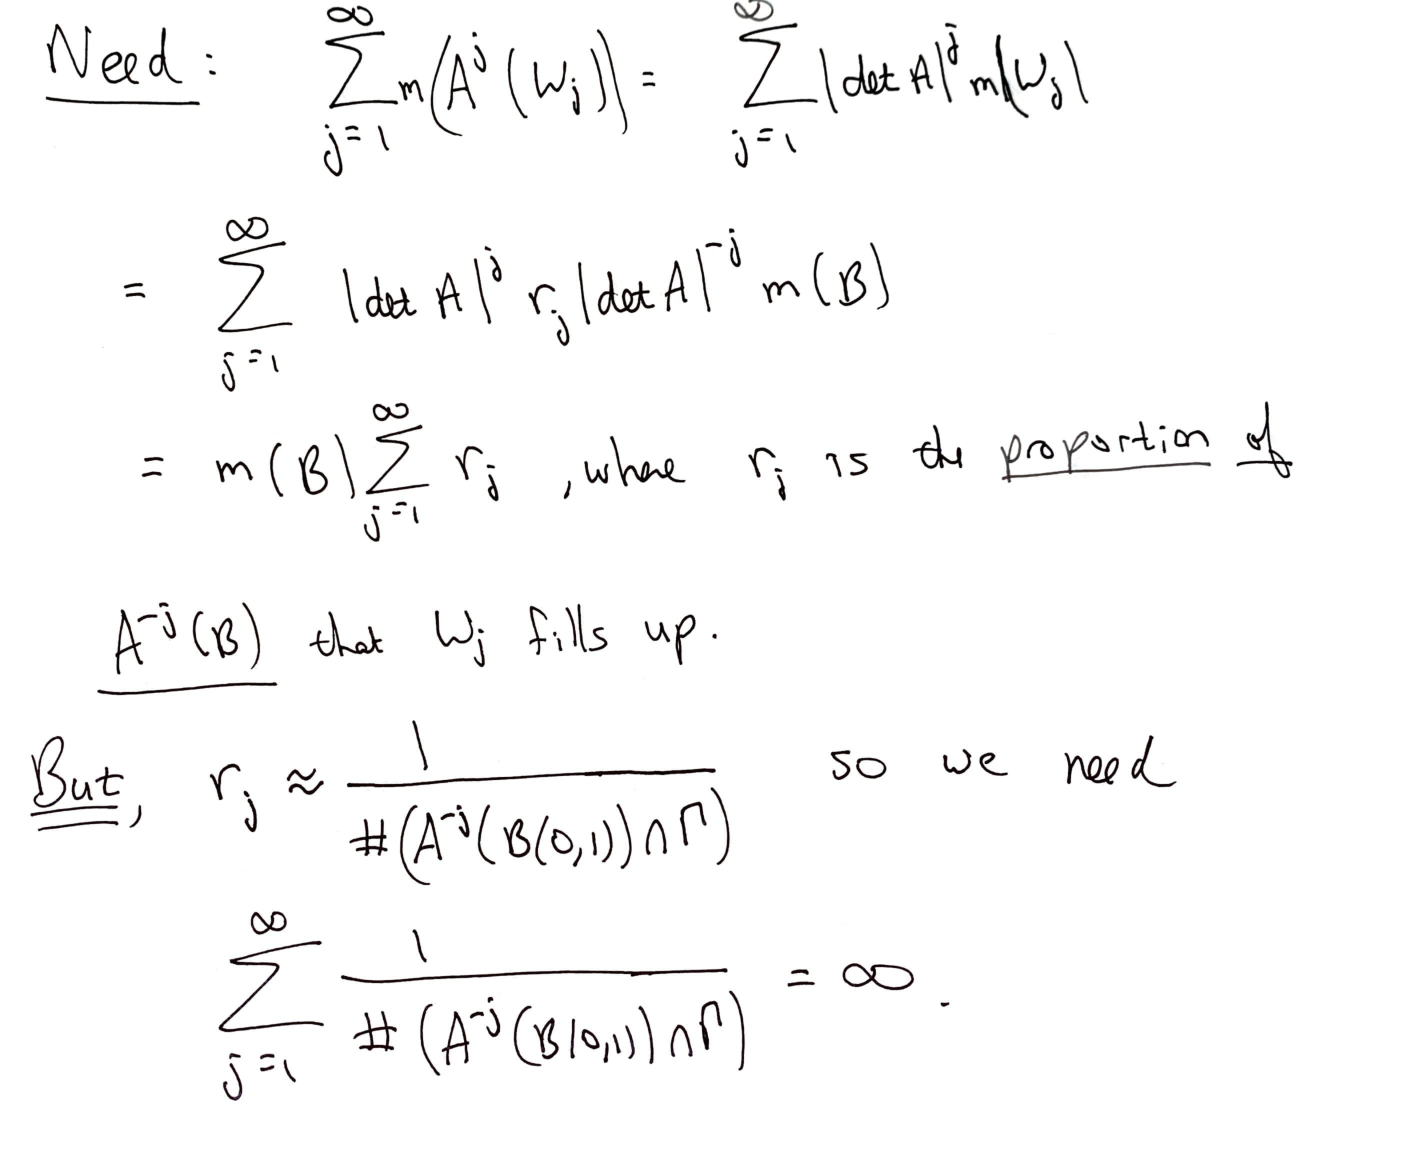
\includegraphics[width=\linewidth,height = 3.3in]{images/obstruction_4.pdf}

\end{frame}



\begin{frame}{Main Result}
   \begin{theorem}
     Let $A$ be an invertible $n \times n$ matrix with $|\det A| > 1$ and $\Gamma$ a full-rank lattice. There exists an $(A, \Gamma)$ wavelet set if and only if 
     \[
       \sum_{j = 1}^\infty \frac {1}{\#\left | A^{-j}(\bb) \cap \Gamma \right |} = \infty
     \]
     
   \end{theorem}
   
   \pause
   
   \begin{remark}
        An obvious corollary is that if 
        \[
        \liminf_{j\to\infty} \#\left | A^{-j}(\bb) \cap \Gamma \right | < \infty,
        \]
        then an $(A, \Gamma)$ wavelet set exists.
   \end{remark}
\end{frame}

\begin{frame}{Relation to Older Results}
    The quantity 
    \[
      \#\left | A^{-j}(\bb) \cap \Gamma \right |
    \]
    has been studied for a relatively long time, often with a continuous parameter $j$ instead of discrete. Of particular interest was the study of when $\#\left | A^{-j}(\bb) \cap \Gamma \right | \to\infty $ as $j \to \infty$. 
    
    \medskip
    
    We next provide some examples of applications where we can apply known results about the ``divergent trajectories."  
\end{frame}

\begin{frame}{Applications}
    \begin{theorem}[Dai-Larson-S, 1997]
    If all eigenvalues of $A$ are greater than 1 in modulus, then there exists an $(A, \Gamma)$ wavelet set.
    \end{theorem}
    
    \begin{proof}
      WLOG assume $\Gamma = \Z^n$.
      
      \medskip
      
      There exists $J$ such that $j \ge J$ implies $A^{-j}(\bb) \subset \bb$. For $j \ge J$, $\#\left | A^{-j}(\bb) \cap \Gamma \right | = 1$ and apply main result.
    \end{proof}
    
\end{frame}

\begin{frame}{Applications}
    \begin{theorem}[Bownik-S, 2021]
    If all eigenvalues of $A$ are greater than {\bf {or equal to}} 1 in modulus, then there exists an $(A, \Gamma)$ wavelet set.
    \end{theorem}
    

    \begin{proof}
      Write $A = \begin{pmatrix}
        A_1 & 0\\ 0& A_2
      \end{pmatrix}
      $, where $A_1$ is expansive and all eigenvalues of $A_2$ are 1 in modulus. Let $T = \begin{pmatrix}  I & 0\\
      0& A_2
      \end{pmatrix}$, and note that all eigenvalues of $T$ are 1 in modulus. 
      
      \medskip
      
      Margulis [1971] showed that if eigenvalues of the matrix $T$ are 1, then $$\liminf_{j \to \infty} \#\left | T^{-j}(\bb) \cap \Gamma \right | < \infty.$$ For large $j$, $A^{-j}(\bb) \subset T^{-j}(\bb)$, which ends the proof.
    \end{proof}
    \end{frame}
    
    
    \begin{frame}
    
    \begin{remark}
       The result in the previous theorem is sharp in the sense that it is the largest set of matrices for which $(A, \Gamma)$ wavelet sets exist for all $\Gamma$. That is, if $|\det A| > 1$ and $A$ has at least one eigenvalue less than 1 in modulus, then there exists $\Gamma$ such that no $(A, \Gamma)$ wavelet set exists.
     \end{remark}
       \bigskip
       \pause
       \begin{remark}
            Bownik and Lemvig proved that if $|\det A| > 1$ and $A$ has at least one eigenvalue less than 1 in modulus, then for almost every full rank lattice $\Gamma$, $(A, \Gamma)$ wavelet sets exist.  
    \end{remark}
    
\end{frame}

\begin{frame}{Applications}
    \begin{theorem}[Ionascu-Wang 2006 (Re-interpreted)]
      Let $n = 2$, $|\det A| > 1$, $\Gamma \subset \R^n$. Assume that one eigenvalue is less than 1 in modulus. TFAE:
      \begin{enumerate}
          \item{1} There exists an $(A, \Gamma)$ wavelet set.
          \item{2} If $X$ is the span of the eigenvector corresponding to the eigenvalue which is less than 1 in modulus, then $X \cap \Gamma = \{0\}$.
          \item{3} $\liminf_{j \to \infty} \#\left | A^{-j}(\bb) \cap \Gamma \right | = 1$
          \item{4} If $\Lambda \subset \Gamma$ and $V = {\mathrm{span}}(\Lambda)$, then 
          \[
          \lim_{j \to \infty} m_V(V \cap A^{-j}(\bb)) < \infty
          \]
          where $m_V$ is Lebesgue measure on $V$.
      \end{enumerate}
    \end{theorem}
\end{frame}

\begin{frame}{Applications}

\begin{theorem}[BS 2021]
   If there exists $\Lambda \subset \Gamma$ such that with $V = \mathrm{span}(\Lambda)$ and 
   \[
   \lim_{j \to \infty} m_V\left (V \cap A^{-j}(\bb)\right) = \infty
   \]
   then there is no $(A, \Gamma)$ wavelet set. Here, as before, $m_V$ is Lebesgue measure on $V$.
\end{theorem}
    
    \pause
    
    \begin{remark}
         The proof of this is complicated. We show instead why the condition of the theorem implies that $\liminf{j\to\infty} \#\left | A^{-j}(\bb) \cap \Gamma \right | = \infty.$
    \end{remark}
\end{frame}

\begin{frame}{Minkowski's First Theorem and Related Result}
      \begin{lemma}
(Minkowski) Let $\Gamma \subset \R^n$ be a full rank lattice, and let $\Omega$ be a symmetric convex body in $\R^n$. Then,
\begin{equation*}
\frac{|\Omega|}{2^n |\R^n/\Gamma|} \le \#|\Omega \cap \Gamma|.
\end{equation*}
In, addition if the vectors $\Omega \cap \Gamma$ linearly span $\R^n$, then
\begin{equation*}
\#|\Omega \cap \Gamma| \le \frac{3^n n! |\Omega|}{2^n |\R^n/\Gamma|}.
\end{equation*}
\end{lemma}
    
    \pause
    
    \begin{remark}
         We only need Minkowski's Theorem to prove the weaker result. The second part of the lemma is used in other parts of the paper.
    \end{remark}
    
\end{frame}

\begin{frame}{Proof}
    Let $\Lambda \subset \Gamma$ be such that (with $V = \mathrm{span}(\Lambda)$),  
   \[
   \lim_{j \to \infty} m_V\left (V \cap A^{-j}(\bb)\right) = \infty.
   \]
    
    By Minkowski's First Theorem, 
    \begin{align*}
            \#|A^{-j}(\bb) \cap \Gamma| &\ge \#|A^{-j}(\bb) \cap \Gamma \cap V|\\
            & \ge C m_V(A^{-j}(\bb) \cap V) \to \infty,
    \end{align*}
    as desired.
    
\end{frame}

\begin{frame}{Special Thanks - Partial List}

\begin{itemize}
    \item Marcin Bownik
    \pause
    \item David Larson
    \pause
    \item Rick Laugesen
    \pause
    \item Qing Gu
    \pause
    \item Barak Weiss
    \pause
    \item Eugen Ionascu and Yang Wang
    \pause
    \item Guido Weiss
\end{itemize}
  
  \medskip\noindent Preprint of ``Simultaneous dilation and translation tilings of $\R^n$" is available on arxiv.
    
\end{frame}


\end{document}

\begin{frame}{Modulus greater than or equal to 1}
\begin{enumerate}
    \item A sufficient condition for an $(A, \Gamma)$ wavelet set to exist is that $\liminf_{j \to \infty} \#\left(A^{-j}(\bb) \cap \Gamma\right) < \infty.$ 
    \item Let $A$ be a matrix whose eigenvalues are all greater than or equal to 1. Write $A$ in real Jordan form as $A = \begin{pmatrix}
      A_1&0\\
      0&A_2
    \end{pmatrix}$ where $A_1$ is expansive and $A_2$ has all eigenvalues equal to 1.
    \item We know there exists $J$ such that $\|A_1^{-j}\| < 1$ for $j \ge J$.
    \item Margulis [1971] showed that $\liminf_{j \to \infty} \#\left(A_2^{-j}(\bb) \cap \Gamma \right) < \infty$, where $\bb$ here is the ball of appropriate dimension relative to $A_2$.
    \item Combine 3 and 4 to see $\liminf_{j \to \infty} \#\left(A^{-j}(\bb) \cap \Gamma\right) < \infty$; conclude $(A, \Gamma)$ wavelet sets exist.
\end{enumerate}
\end{frame}

\begin{frame}{Higher Dimension Poll}

All of these are equivalent in 2-d. Pairs which satisfy 3 but not 2 are {\it {non-trivial divergent trajectories}}. Which condition is equivalent to existence of wavelet sets in $\R^n$?

\begin{enumerate}
    \item $\liminf_{j \to \infty} \#|A^{-j}(\bb) \cap \Gamma| = 1$
    \item $\liminf_{j \to \infty} \#|A^{-j}(\bb) \cap \Gamma| < \infty$
    \item For every sublattice $\Lambda \subset \Gamma$, if $V = {\mathrm {span}}(\Lambda)$ and $d$ is the dimension of $V$, then 
    \[
    \liminf_{j\to \infty} m_d(V \cap A^{-j}(\bb)) < \infty
    \]
    where $m_d$ is $d$-dimensional Lebesgue measure.
    \item Let $X$ be the space spanned by the eigenvectors associated with eigenvalues with modulus less than 1. Then $X \cap \Gamma = \{0\}$.
\end{enumerate}
\end{frame}

\begin{frame}{PLOT TWIST!}
    None of them, LOL. The following condition is in-between conditions (2) and (3) from the previous slide.
    \begin{theorem}[Bownik-S 2021]
      There exists an $(A, \Gamma)$ wavelet set if and only if
      \[
      \sum_{j = 1}^\infty \frac {1}{\#\left(A^{-j}(\bb) \cap \Gamma\right)} = \infty
      \]
    \end{theorem}
\end{frame}

\begin{frame}{Some results in higher dimensions}
\begin{enumerate}
    \item If $\liminf_{j \to \infty} \#\left(A^{-j}(\bb) \cap \Gamma \right) < \infty$, then $(A, \Gamma)$ wavelet sets exist (BS)
    \item If at least one eigenvalue is less than 1 in modulus, then there is a lattice $\Gamma$ such that $(A, \Gamma)$ does not have a wavelet set, but for almost every lattice $\Gamma$, an $(A,\Gamma)$ wavelet set exists. (Bownik-Lemvig)
    \item If there is a sublattice $\Lambda \subset \Gamma$ with $V = {\mathrm {span}}(\Lambda)$ and $d$ the dimension of $V$ such that
    \[
    \lim_{j\to \infty} m_d(V \cap A^{-j}(\bb)) = \infty
    \]
    where $m_d$ is $d$-dimensional Lebesgue measure, then $\liminf_{j \to \infty} \#\left(A^{-j}(\bb) \cap \Gamma \right) = \infty$ (Minkowski)
    \item There exists a pair $(A, \Gamma)$ such that for all lattice subspaces $V$, $ \liminf_{j\to \infty} m_d(V \cap A^{-j}(\bb)) < \infty$, but $\lim_{j \to \infty} \#\left(A^{-j}(\bb) \cap \Gamma \right) = \infty$ (Khinchine) 
\end{enumerate}
    
\end{frame}





\begin{frame}{Obstruction to Existence of Wavelets 1/4}

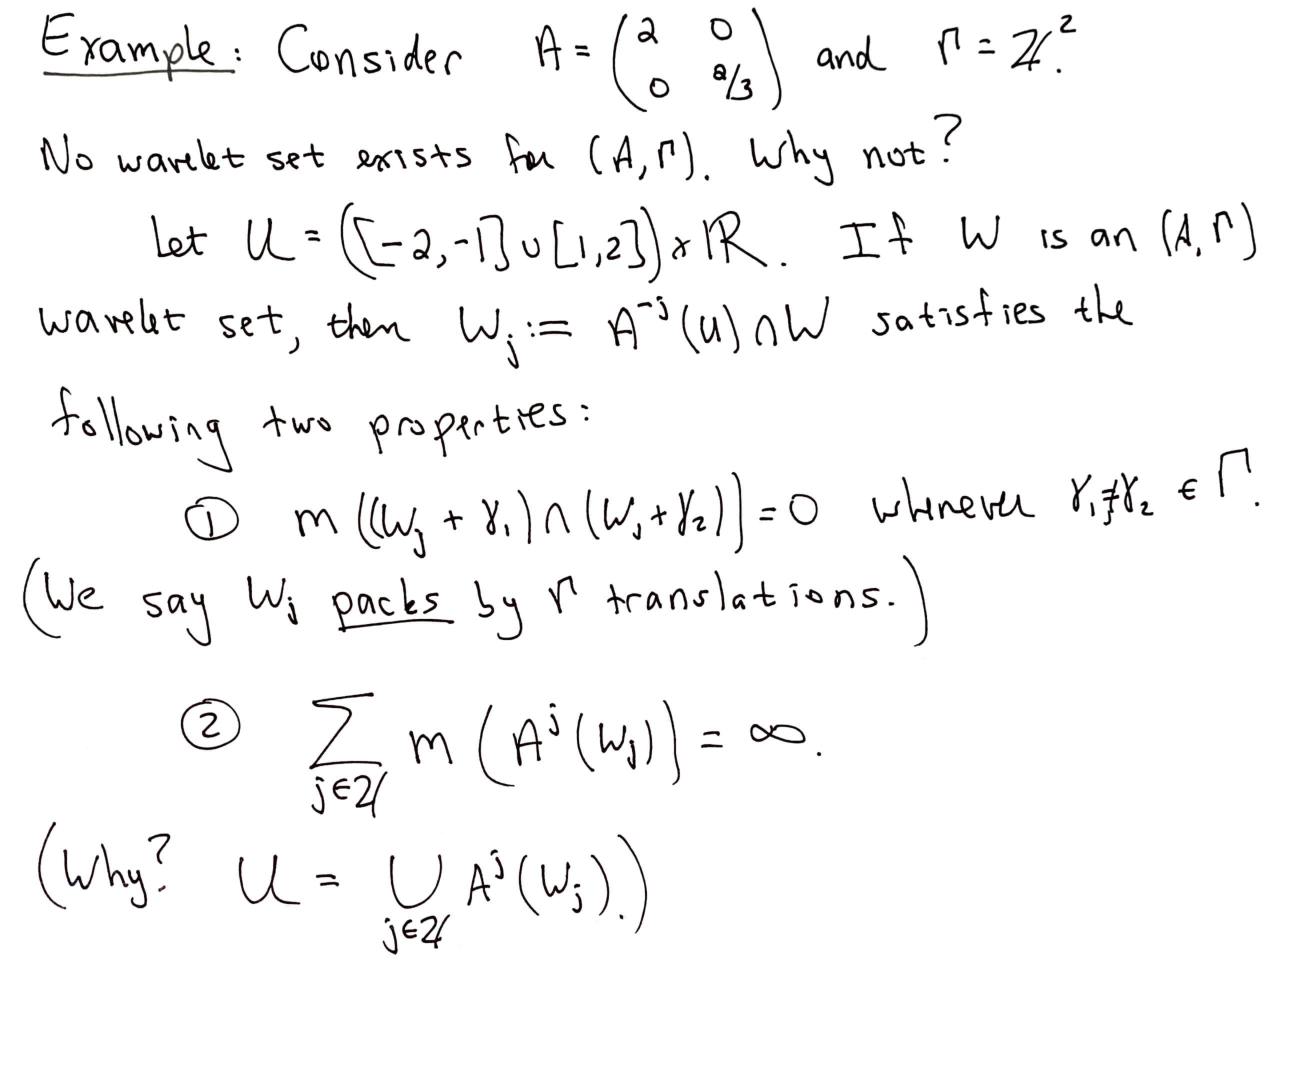
\includegraphics[width=\linewidth,height = 3.4in]{images/obstruction_1.pdf}

    
\end{frame}

\begin{frame}{Obstruction to Existence of Wavelets 2/4}

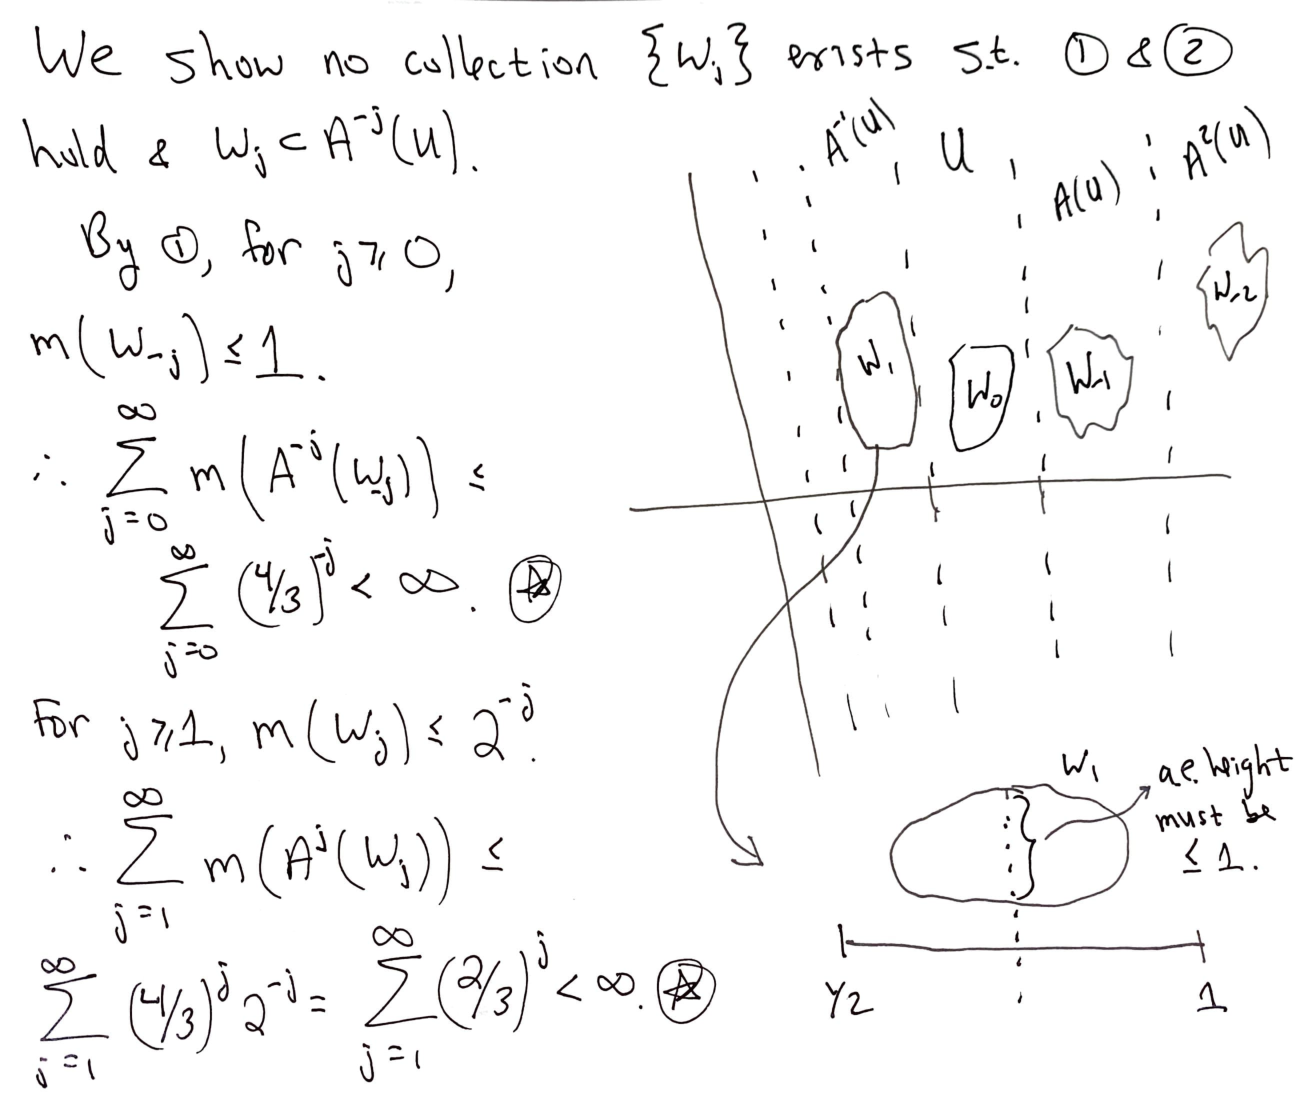
\includegraphics[width=\linewidth,height = 3.1in]{images/obstruction_2.pdf}

    
\end{frame}

\begin{frame}{Obstruction to Existence of Wavelets 3/4}

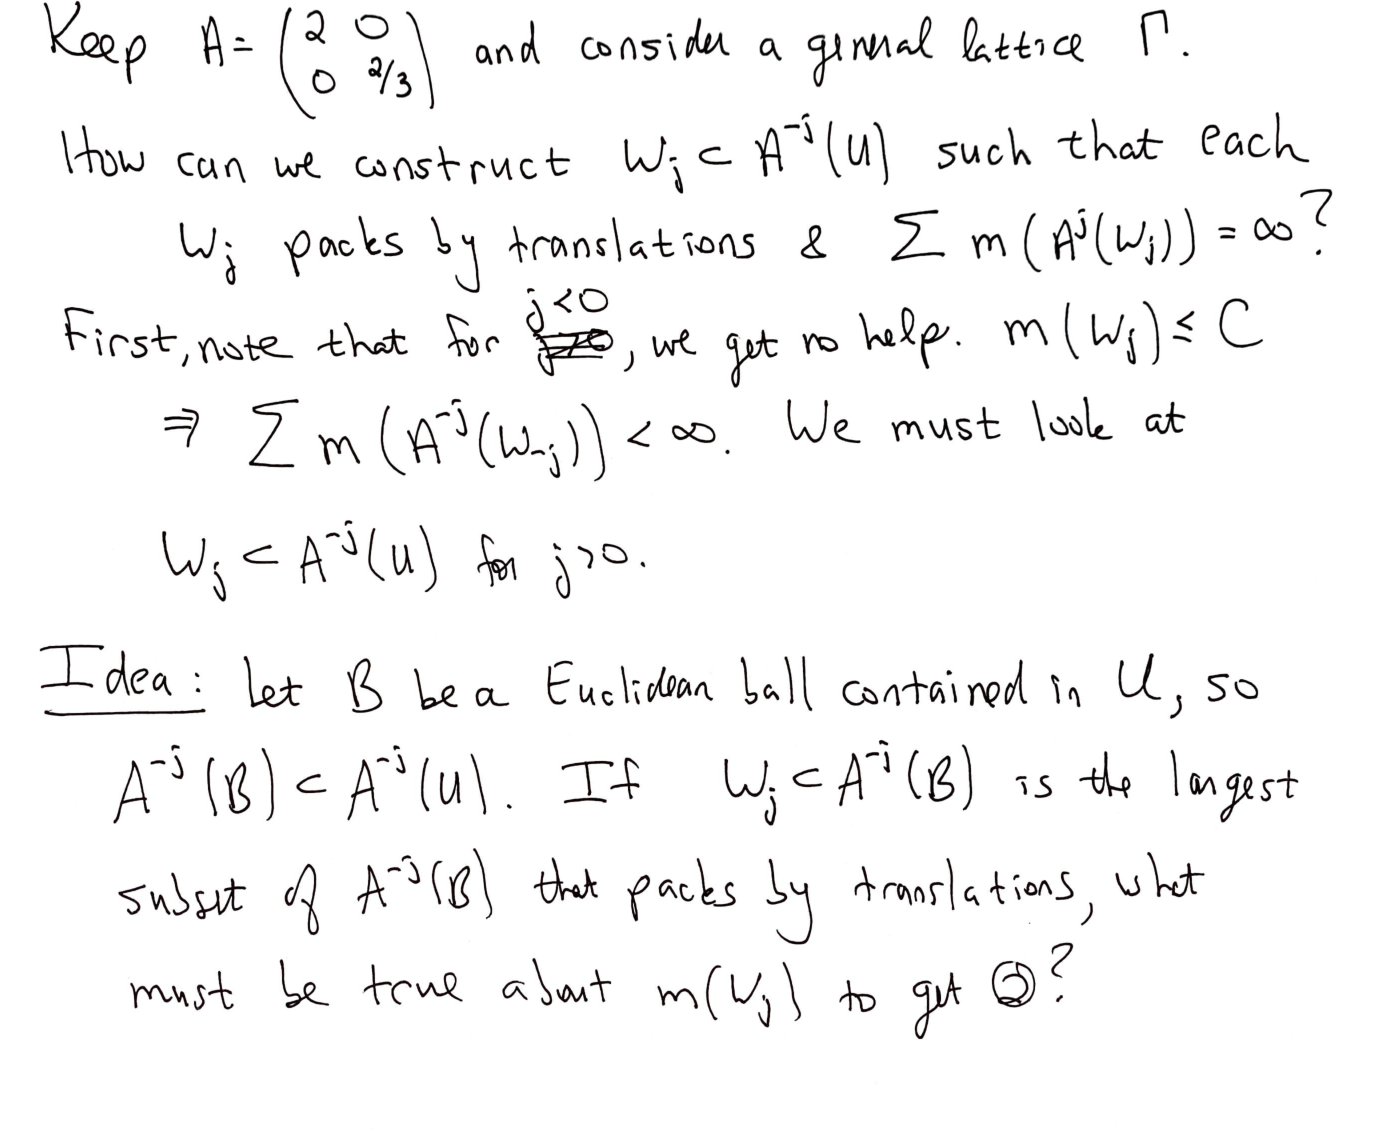
\includegraphics[width=\linewidth,height = 3.3in]{images/obstruction_3.pdf}

    
\end{frame}

\begin{frame}{Obstruction to Existence of Wavelets 4/4}

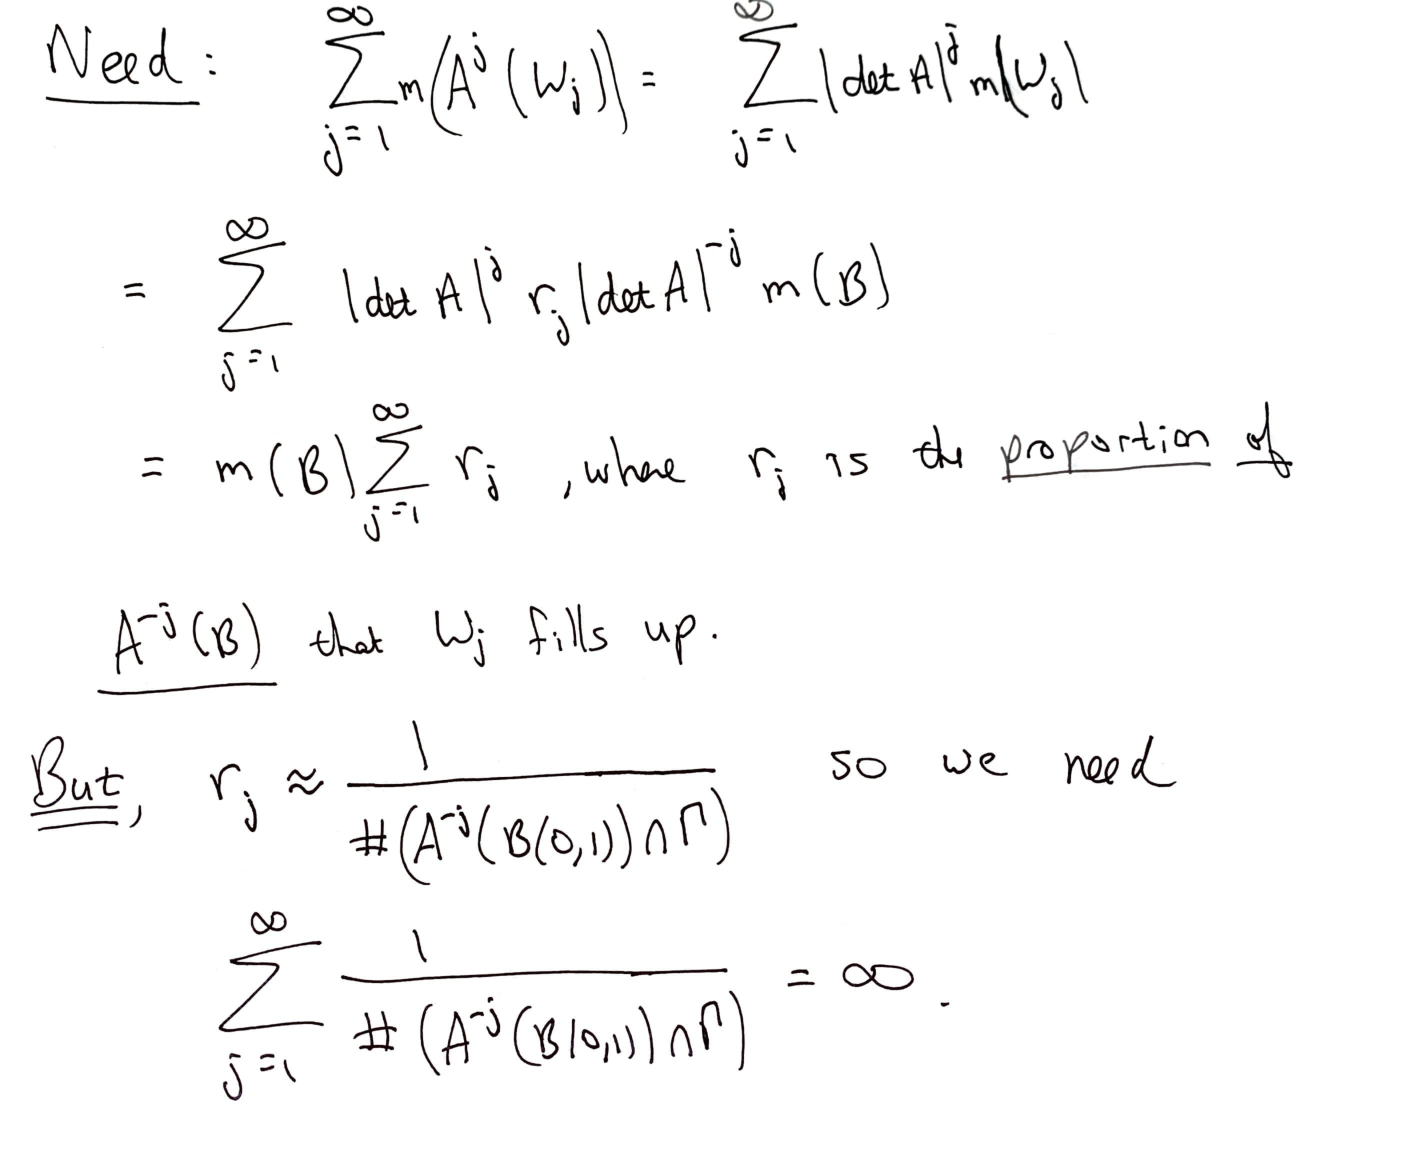
\includegraphics[width=\linewidth,height = 3.3in]{images/obstruction_4.pdf}

    
\end{frame}